\documentclass[11pt]{article}

\usepackage[a4paper,margin=1in]{geometry}
\usepackage{microtype}
\usepackage{mathtools,amssymb}
\usepackage{tikz}
\usetikzlibrary{arrows.meta,calc,fit,positioning}
\usepackage[hidelinks]{hyperref}

\title{Datra primer}
\author{\texttt{@qualiascript} \and ChatGPT}
\date{}

\newcommand{\code}[1]{\texttt{#1}}
\newcommand{\StaDaTraMon}{\mathsf{StaDaTraMon}}
\newcommand{\HorSum}{\boxplus}

\tikzset{
  atlas node/.style={draw,rounded corners=2pt,minimum height=7mm,
    minimum width=16mm,inner sep=3pt,fill=blue!4},
  selected node/.style={atlas node,fill=orange!12},
  atlas arrow/.style={-{Stealth[length=2mm]},semithick},
  morphism arrow/.style={-{Stealth[length=2mm]},thick,orange!75!black},
  page label/.style={font=\small\sffamily,text=black!65},
  atlas label/.style={font=\small\itshape,text=black!70},
}

\begin{document}
\maketitle

This post is meant to serve as context and intuition-building for the
\href{run:preprint.pdf}{Datra preprint}, and as such, it will take a
different approach to Datra. We will be focusing on the
\(\StaDaTraMon\) monoidal category, but instead of introducing it in
technical terms, I will illustrate the ideas underpinning the design of the
Datra programming language. I will start from the original vision, wherein
Datra was supposedly a language where ``everything is a map''. This idea has
not survived the final design, however, the idea of maps is still central to
Datra and serves as a useful starting point.

Let us define sets \(A = \{1, 4, 7\}\), \(B = \{2, 3, 5\}\),
\(C = \{6, 8, 9\}\). Then, \(\code{[[A; B]; C]}\) serves as a Datra map,
which is distinct from \(\code{[A; [B; C]]}\), \(\code{[B; C; A]}\) or
other maps with the same underlying data but a different presentation. That
    is because, for instance,
    \code{[[A := 1;\allowbreak\ B := 5];\allowbreak\ C := 8]} serves as
an inhabitant of the original map, but not of the other maps, despite
obviously being able to be turned into an inhabitant of the maps with the
same data. We also consider map \(\code{[[A; B]; C; []]}\), where
\(\code{[]}\) holds no data, however, we deem this map as equivalent to
\(\code{[[A; B]; C]}\) by definition. The map \(\code{[A; [B; C]]}\) can
be viewed as a tree, in the following manner:

\begin{figure}[htbp]
\centering
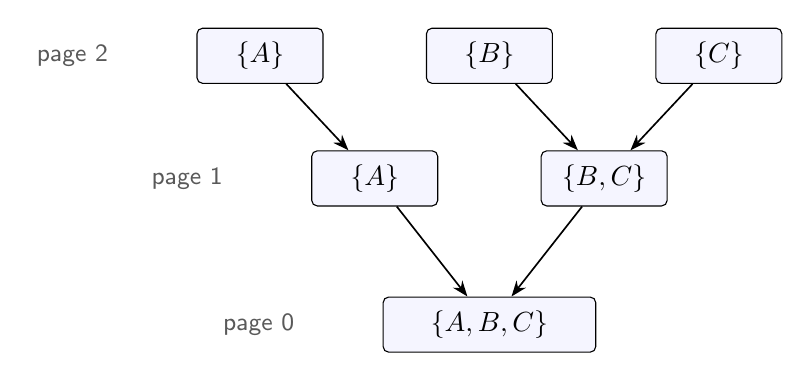
\begin{tikzpicture}[node distance=12mm and 13mm]
  \node[atlas node] (a2) {\(\{A\}\)};
  \node[atlas node,right=of a2] (b2) {\(\{B\}\)};
  \node[atlas node,right=of b2] (c2) {\(\{C\}\)};
  \node[atlas node,below=of $(a2)!0.5!(b2)$] (a1) {\(\{A\}\)};
  \node[atlas node,below=of $(b2)!0.5!(c2)$] (bc1) {\(\{B,C\}\)};
  \node[atlas node,below=15mm of $(a1)!0.5!(bc1)$,
    minimum width=27mm] (abc0) {\(\{A,B,C\}\)};
  \draw[atlas arrow] (a2) -- (a1);
  \draw[atlas arrow] (b2) -- (bc1);
  \draw[atlas arrow] (c2) -- (bc1);
  \draw[atlas arrow] (a1) -- (abc0);
  \draw[atlas arrow] (bc1) -- (abc0);
  \node[page label,left=10mm of a2] {page 2};
  \node[page label,left=10mm of a1] {page 1};
  \node[page label,left=10mm of abc0] {page 0};
\end{tikzpicture}
\caption{The pagination of \(\code{[A; [B; C]]}\).}
\label{fig:pagination}
\end{figure}

Things to note in this tree structure: its cardinality is the height of the
three, in this case, \(3\), from \(0\) to \(2\). The collection of nodes at
each height level is considered a page, and by extension, the shape of the
three, without the data underlying it, is considered a pagination. At page
\(0\), the tree has only one node, whose underlying data we consider the
\textbf{extent} of the DaTra type. The nodes on the last page are considered
the \textbf{territory}. The nodes on each page are ordered, and the edges
between nodes respect this ordering, as we established previously, despite
any ordering having isomorphic data. Going from a node on page \(x\) to page
\(x - 1\), the edge must represent an injection, as we retrieve some, but
not necessarily all, of the data. Furthermore, the images of these
injections ought to be pairwise disjoint in the target, as to not generate
new data that was not available in the extent.

For the tree structure to represent a map, there is another requirement: the
territory must match the extent, as in, all data in the extent mus recall
that t be represented by an argument of the territory. Otherwise, the
supposed map would have inaccessible ``hidden'' data, not represented by its
literal notation, such as \(\code{[A; [B; C]]}\). This is, however,
completely fine, as long as we do not take for granted that the structure
must represent a map. An alternative view would be to see the tree structure
as representing the different presentations of some data at different
pages, allowing for data loss in the process. This is a useful generalization
of the concept, and one that we will take. Furthermore, given any atlas, one
can recover a map from it by using the Charting functor, as detailed in the
preprint.

Another issue to consider is size. In this example, everything is finite,
but this is not necessarily the case. However, we also seek to avoid data
that is too large to handle in concrete, computational terms. The solution
taken is as follows: all the data at any node is to be countable, and each
node is to have a countable number of nodes in the page above that point to
it. The cardinality, that is, number of pages, is finite, however, we will
find ourselves in the situation of asking for the data at a page number
higher than the cardinality. In that case, we consider that the final page
repeats. The nodes at each page are still ordered, however, they are not
ordered merely by positive integers, but by ordinals smaller than
\(\omega_0^{\omega_0}\). This convention allows the ordering of nodes even
after a countably infinite number of nodes are introduced.

To be specific, the data structure we have introduced so far is an atlas
object, by the terminology of the preprint. An object in
\(\StaDaTraMon\) can represent multiple atlas objects, by usual sum types
logic. Atlas morphisms are flexible, but morphisms in \(\StaDaTraMon\) are
more restrictive. Let us look at the case of two atlas objects represented
by \(\StaDaTraMon\) and a morphism between the two. The rules are as follows:
each node from the origin atlas must be sent to a node of the target atlas,
so that the function between atlas nodes is injective. The extent of the
origin atlas must be sent to the target of the origin atlas. The ordering of
nodes must be preserved, in the following sense: given any two nodes of the
origin atlas, we can find whether one is to the left of the other by pulling
back at a common page. Then, the morphism must respect this order in the
image, as well. Each origin node sent to a target node must induce an
injection between the data at the two nodes, that is, each node is sent to a
node with more or equal data. Finally, for any node in the origin, if it has
a territory in the final page that it is the image of, then this must be
preserved by the morphism. Each of these rules can be relaxed by moving to a
different category than \(\StaDaTraMon\), however, all these rules are
imposed in \(\StaDaTraMon\) itself.

    To illustrate why these rules are helpful, consider a morphism
from \(\code{*}\) to \(\code{[A; [B; C]]}\), where \(\code{*}\) is the
atlas given by a tree with cardinality \(1\) and whose extent is the
singleton set. In this case, a morphism picks an element of \(A\), \(B\) or
\(C\), thus viewing the map as a sum type. Also consider, for any atlas map,
a morphism from the map with the same pagination, but whose territories are
all singleton. In this case, the morphism selects an element of each of the
values of the map, while remembering the full data. For instance,
    \code{[A := 7;\allowbreak\ [B := 2;\allowbreak\ C := 6]]} can be
    denoted as one of those
morphisms.

\begin{figure}[htbp]
\centering
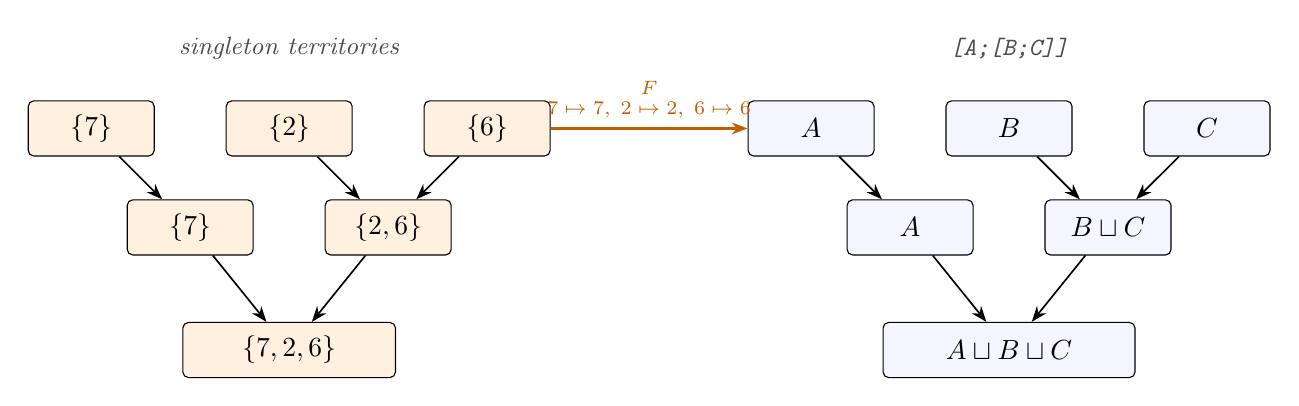
\begin{tikzpicture}[node distance=9mm and 9mm]
  % Source atlas
  \node[selected node] (sA) {\(\{7\}\)};
  \node[selected node,right=of sA] (sB) {\(\{2\}\)};
  \node[selected node,right=of sB] (sC) {\(\{6\}\)};
  \node[selected node,below=of $(sA)!0.5!(sB)$] (s7) {\(\{7\}\)};
  \node[selected node,below=of $(sB)!0.5!(sC)$] (s26) {\(\{2,6\}\)};
  \node[selected node,below=12mm of $(s7)!0.5!(s26)$,
    minimum width=27mm] (sall) {\(\{7,2,6\}\)};
  \draw[atlas arrow] (sA)--(s7); \draw[atlas arrow] (sB)--(s26);
  \draw[atlas arrow] (sC)--(s26); \draw[atlas arrow] (s7)--(sall);
  \draw[atlas arrow] (s26)--(sall);
  \node[atlas label,above=4mm of sB] {singleton territories};

  % Target atlas
  \node[atlas node,right=25mm of sC] (tA) {\(A\)};
  \node[atlas node,right=of tA] (tB) {\(B\)};
  \node[atlas node,right=of tB] (tC) {\(C\)};
  \node[atlas node,below=of $(tA)!0.5!(tB)$] (ta) {\(A\)};
  \node[atlas node,below=of $(tB)!0.5!(tC)$] (tbc) {\(B\sqcup C\)};
  \node[atlas node,below=12mm of $(ta)!0.5!(tbc)$,
    minimum width=32mm] (tall) {\(A\sqcup B\sqcup C\)};
  \draw[atlas arrow] (tA)--(ta); \draw[atlas arrow] (tB)--(tbc);
  \draw[atlas arrow] (tC)--(tbc); \draw[atlas arrow] (ta)--(tall);
  \draw[atlas arrow] (tbc)--(tall);
  \node[atlas label,above=4mm of tB] {\(\code{[A;[B;C]]}\)};

  % The nodewise atlas morphism, summarized between the two trees.
  \draw[morphism arrow] (sC.east) -- node[above,align=center,font=\scriptsize]
    {\(F\)\\[-1pt]\(7\mapsto7,\;2\mapsto2,\;6\mapsto6\)} (tA.west);
\end{tikzpicture}
\caption{The atlas morphism denoted by
  \(\code{[A := 7; [B := 2; C := 6]]}\). Orange nodes carry the selected
  singleton data; the horizontal arrow summarizes its nodewise injections.}
\label{fig:selected-morphism}
\end{figure}

As such, Datra semantics support partial and total maps, as well as canonical
map orderings. By using multiple atlases and imposing a coherence condition,
it can also represent maps who's some of the arguments admit multiple
orders. Part of the underlying data can also include argument names,
represented by identifier strings that depend on values. This ties with
another concept for Datra: a language for partially named partial maps with
partially variable argument order. However, even this is a mere facet of
Datra semantics, which are flexible enough to model various aspects of data
modeling, function call semantics, config files and other programmatic
aspects which fall into the broad category of ``data transformations''. In
particular, by dropping the map requirements, an atlas can also model the
results of computation at different stages, so that this unifies maps and
functions within the same semantics.

The so-called ``horizontal sum'' operator, \(\HorSum\), takes two
\(\StaDaTraMon\) morphisms and puts them side by side. It can be seen as
the operation of merging two trees by letting the extent be the coproduct
of their respective extents, and each page above 0 being composed of the
pages of the trees at the respective level. This operation is closely
related to the map-creating operation, for instance, one can construct
\(\code{[B := 2; C := 6]}\) out of \((B := 2) \HorSum (C := 6)\).
However, the map semantics instead keep the extents of the trees on
page 1 of the new tree. Below is a representation of the horizontal sum
operation on \((B := 2) \HorSum (C := 6)\).

\begin{figure}[htbp]
\centering
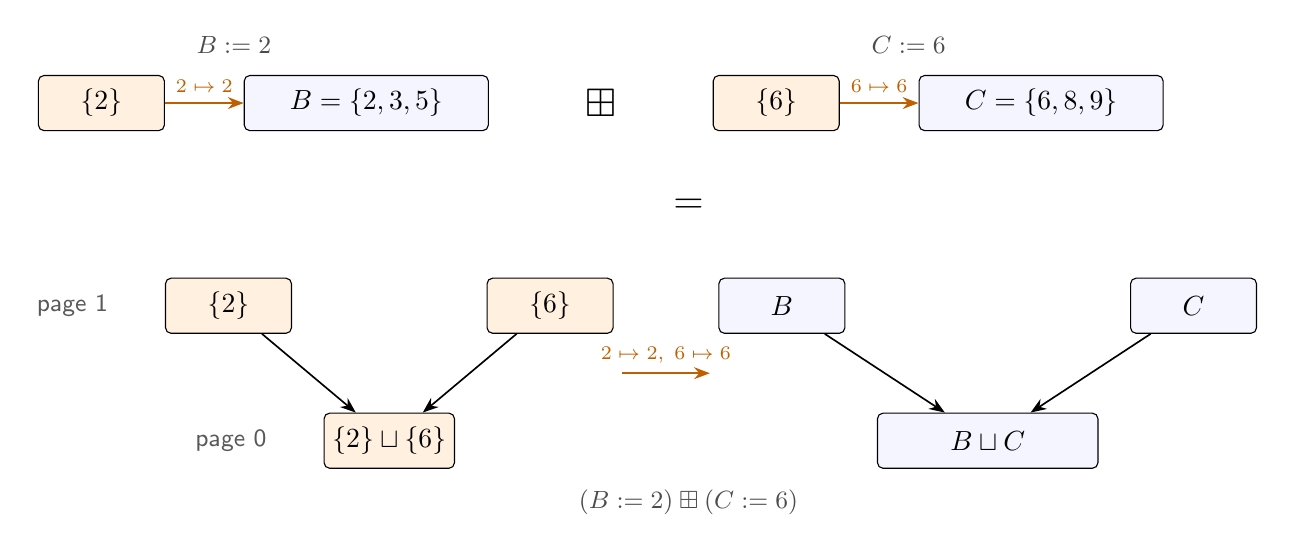
\begin{tikzpicture}[node distance=10mm and 10mm]
  % Each operand is a morphism between one-node atlases.
  \node[selected node] (bsource) {\(\{2\}\)};
  \node[atlas node,right=of bsource,minimum width=31mm] (btarget)
    {\(B=\{2,3,5\}\)};
  \draw[morphism arrow] (bsource)--node[above,font=\scriptsize]
    {\(2\mapsto2\)} (btarget);
  \node[atlas label,above=5mm of $(bsource)!0.5!(btarget)$]
    {\(B := 2\)};

  \node[font=\Large,right=11mm of btarget] (plus) {\(\HorSum\)};

  \node[selected node,right=11mm of plus] (csource) {\(\{6\}\)};
  \node[atlas node,right=of csource,minimum width=31mm] (ctarget)
    {\(C=\{6,8,9\}\)};
  \draw[morphism arrow] (csource)--node[above,font=\scriptsize]
    {\(6\mapsto6\)} (ctarget);
  \node[atlas label,above=5mm of $(csource)!0.5!(ctarget)$]
    {\(C := 6\)};

  \node[font=\Large,below=11mm of $(plus)!0.5!(csource)$] (equals) {\(=\)};

  % The sum has one coproduct extent and tagged copies of both positive pages.
  \node[selected node,below=24mm of equals,xshift=-38mm] (rsourceall)
    {\(\{2\}\sqcup\{6\}\)};
  \node[selected node,above left=10mm and 4mm of rsourceall] (rsourceb)
    {\(\{2\}\)};
  \node[selected node,above right=10mm and 4mm of rsourceall] (rsourcec)
    {\(\{6\}\)};
  \draw[atlas arrow] (rsourceb)--(rsourceall);
  \draw[atlas arrow] (rsourcec)--(rsourceall);

  \node[atlas node,below=24mm of equals,xshift=38mm,minimum width=28mm]
    (rtargetall) {\(B\sqcup C\)};
  \node[atlas node,above left=10mm and 4mm of rtargetall] (rtargetb) {\(B\)};
  \node[atlas node,above right=10mm and 4mm of rtargetall] (rtargetc) {\(C\)};
  \draw[atlas arrow] (rtargetb)--(rtargetall);
  \draw[atlas arrow] (rtargetc)--(rtargetall);

  % As in Figure 2, one arrow summarizes the nodewise morphism.
  \node[fit=(rsourceb)(rsourcec)(rsourceall),inner sep=1mm] (rsource) {};
  \node[fit=(rtargetb)(rtargetc)(rtargetall),inner sep=1mm] (rtarget) {};
  \draw[morphism arrow] (rsource.east)--node[above,font=\scriptsize]
    {\(2\mapsto2,\;6\mapsto6\)} (rtarget.west);

  \node[page label,left=6mm of rsourceb] {page 1};
  \node[page label,left=6mm of rsourceall] {page 0};
  \node[atlas label,below=5mm of $(rsourceall)!0.5!(rtargetall)$]
    {\((B := 2) \HorSum (C := 6)\)};
\end{tikzpicture}
\caption{Each operand is a morphism between one-node atlases. Their
horizontal sum forms a single coproduct extent on page \(0\), while page
\(1\) contains the two operand pages side by side. The orange arrow
summarizes the nodewise injections of the summed morphism.}
\label{fig:horizontal-sum}
\end{figure}

I believe that there are many other interesting aspects of Datra semantics
to explore, which become easier to comprehend as part of an actual
programming language, rather than as manually-explained facets of the
mathematical model of the language's semantics. This document serves as an
explanation for the design principles underlying Datra, not a comprehensive
explanation of the language's semantics and capabilities. For instance,
there ought to be a way to model Python-style \(\code{kargs}\) /
\(\code{kwargs}\) as first-class Datra constructions, however, this is
beyond the scope of this document. The eventual construction of advanced
Datra features is best kept within the actual Datra programming language,
which I believe \(\StaDaTraMon\) has enough flexibility to model in a
type-safe manner.

\end{document}
